\begin{figure}[t]
  \centering
  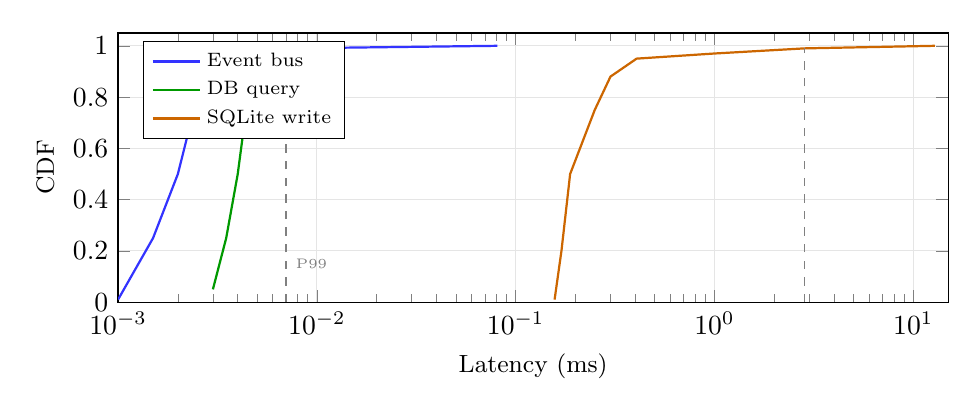
\begin{tikzpicture}
    \begin{axis}[
      width=\columnwidth,
      height=5cm,
      xlabel={Latency (ms)},
      ylabel={CDF},
      ylabel style={font=\small},
      xlabel style={font=\small},
      xmode=log,
      xmin=0.001, xmax=15,
      ymin=0, ymax=1.05,
      ytick={0,0.2,0.4,0.6,0.8,1.0},
      grid=major,
      grid style={gray!20},
      legend style={at={(0.03,0.97)}, anchor=north west, font=\scriptsize},
      legend cell align=left,
      every axis plot/.append style={thick, no markers},
    ]
    % Event bus dispatch (P50=0.002, P95=0.003, P99=0.007, max=0.081)
    \addplot[blue!80] coordinates {
      (0.001,0.01) (0.0015,0.25) (0.002,0.50)
      (0.0025,0.80) (0.003,0.95) (0.005,0.98)
      (0.007,0.99) (0.081,1.0)
    };
    \addlegendentry{Event bus}

    % DB query (P50=0.004, P95=0.005, P99=0.006)
    \addplot[green!60!black] coordinates {
      (0.003,0.05) (0.0035,0.25) (0.004,0.50)
      (0.0045,0.80) (0.005,0.95) (0.0055,0.98)
      (0.006,0.99) (0.01,1.0)
    };
    \addlegendentry{DB query}

    % SQLite task write (P50=0.188, P95=0.406, P99=2.839, max=12.83)
    \addplot[orange!80!black] coordinates {
      (0.157,0.01) (0.170,0.20) (0.188,0.50)
      (0.250,0.75) (0.300,0.88) (0.406,0.95)
      (1.0,0.97) (2.839,0.99) (12.83,1.0)
    };
    \addlegendentry{SQLite write}

    % P99 reference lines
    \draw[gray, thin, dashed] (axis cs:0.007,0) -- (axis cs:0.007,0.99)
      node[pos=0.15, right, font=\tiny, text=gray] {P99};
    \draw[gray, thin, dashed] (axis cs:2.839,0) -- (axis cs:2.839,0.99);

    \end{axis}
  \end{tikzpicture}
  \caption{CDF of intra-platform latency for critical data paths
  (1{,}000 iterations each, log-scale x-axis).  Event bus dispatch
  and DB queries complete in under 10\,$\mu$s at P99.
  SQLite writes reach P99 at 2.84\,ms.  LLM schedule generation
  (not shown; P50 = 6.3\,s) operates on a per-day cadence.}
  \label{fig:latency-cdf}
\end{figure}
